Para la problemática presentada anteriormente presentamos en esta sección: el objetivo, objetivos específicos, la justificación, el alcance y la descripción de la propuesta de solución.\\

%Definir correspondencia

\section{Objetivo}

Para mitigar las causas y reducir el impacto de los problemas que se tienen nos basamos en el siguiente objetivo: \\

Desarrollar e implementar una aplicación web para el apoyo en el control de la correspondencia del CMPL. \\

\subsection{Objetivos Específicos}

\begin{itemize}
	\item Cubrir los lineamientos establecidos para el control de correspondencia en el Manual de Procedimientos del CMPL.
	\item Tener un respaldo electrónico de los oficios y memorándums para posterior consulta.
	\item Llevar un registro de los oficios entrantes y salientes.
	\item Notificar al personal que tiene correspondencia por atender.
	\item Dar seguimiento a los asuntos que se deben atender.
\end{itemize}

\section{Justificación}
Con este trabajo se mitigarán las causas de algunos de los problemas mencionados como: que el registro de los oficios se lleve de manera adecuada, se tenga un respaldo digital del oficio, que se restringa el acceso a la información confidencial al personal indicado, que se pueda saber a quien se le turna un oficio y a quien se le envía copia, saber el momento en que se respondió, saber si requiere respuesta, saber si el asunto ya fue atendido, saber quien lo entregó, saber quien lo registró, informar a la persona que se le turna que tiene un asunto por atender, que los oficios sean validados, saber la ubicación física de los oficios, además de que cumpliran con la normatividad. Pero sí continua, el rezago tecnológico va a ser necesario que el CMPL adquiera nuevos equipos y que capacite a su personal. \\
%De acuerdo con los objetivos anteriores 
%Desarrollar e implementar una aplicación web que fortalezca los procesos de la administración del CMPL.

\section{Alcance}

Para presentar de mejor manera el alcance de la aplicación se divide de la siguiente manera: \\

\begin{itemize}
	\item Funcionalidad: muestra los módulos por los que estará formado la aplicación y los diferentes tipos de usuarios que la utilizarán.
	\item Plataforma: el hardware, el software y los servicios necesarios para la aplicación.
	\item Procedimiento: descripción y mejoras al procedimiento anterior.
	\item Información: la información que se va a manejar dentro de la aplicación.
	\item Propiedades de software: son los atributos con los que contará la aplicación.
	\item Interacción con el usuario: la forma en que el usuario podrá hacer el intercambio de información con la aplicación.
\end{itemize}

%%%%%%%%%% FUNCIONALIDAD %%%%%%%%%%%%
%%%%%%%%%%%%%%%%%%%%%%%%%%%%%%%%%%%%%

\subsection{Funcionalidad}

La funcionalidad la aplicación se organizará de la siguiente manera: un módulo para la gestión de usuarios, un modulo para la correspondencia interna, un módulo para la correspondencia externa. En la figura \ref{diagrama a bloques} se puede ver de manera más precisa como interactuan los bloques anteriores con los diferentes tipos de usuarios.\\

	\begin{figure}[htbp!]
		\centering
			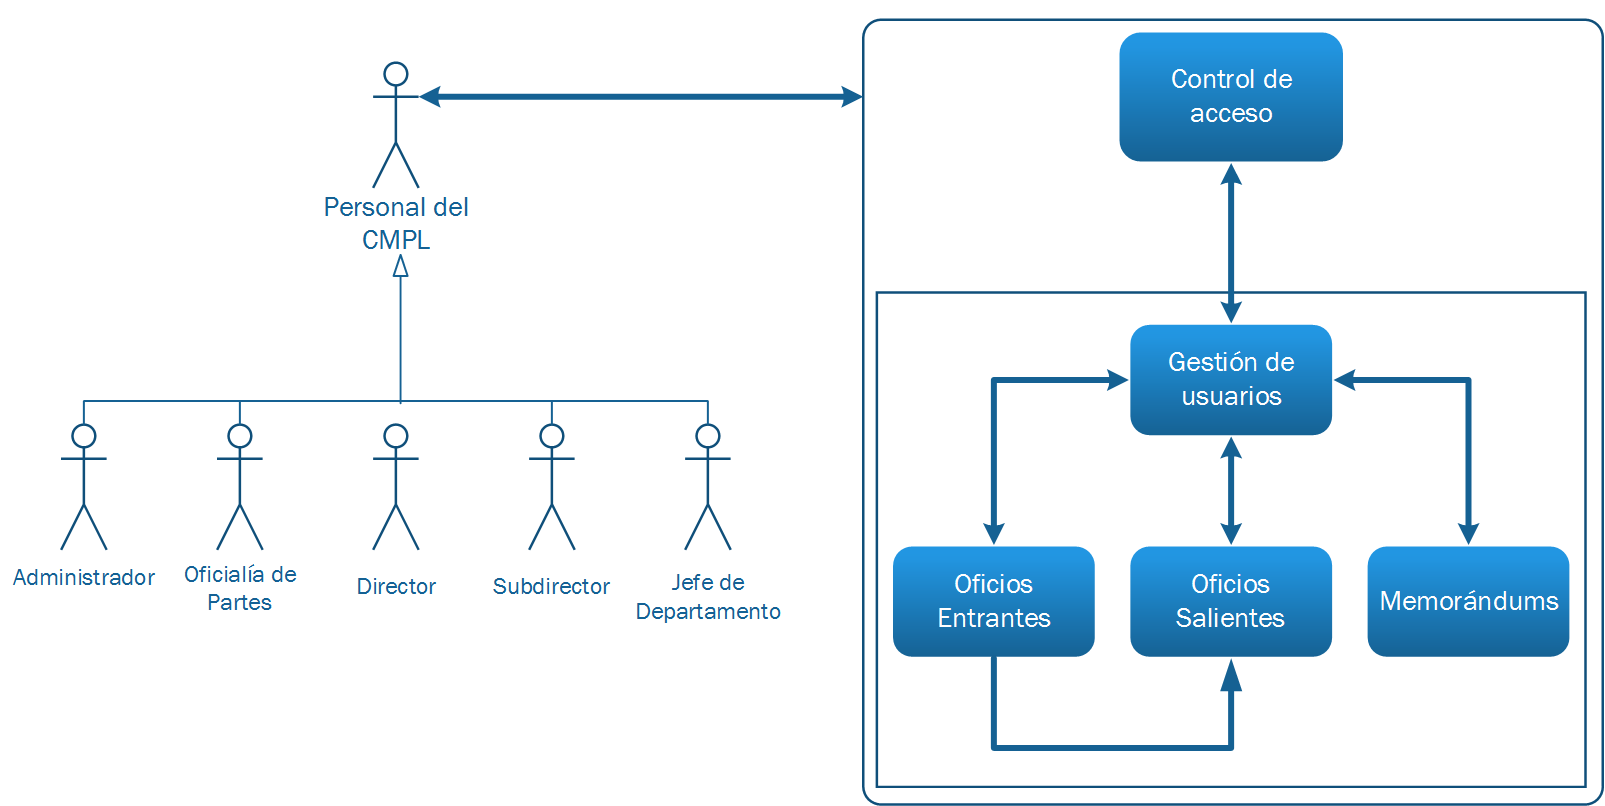
\includegraphics[width=0.8\textwidth]{images/propuesta/diagramabloques}
		\caption{Diagrama de Bloques de la Aplicación.}
		\label{diagrama a bloques}
	\end{figure}

A continuación se describe cada módulo.

\subsubsection{Módulo 1: Gestión de usuarios}
Este modulo permitirá el registro, la consulta, los cambios y la baja de usuarios; además permitirá el control de acceso a la aplicación para que los usuarios puedan hacer uso de la misma. \\
 
Los requerimientos considerados para este módulo son los siguientes:
\begin{itemize}
	\item El usuario necesita tener una nombre de usuario y una contraseña.
	\item El usuario necesita editar sus datos.
	\item El usuario necesita un mecanismo para recuperar su contraseña.
	\item El usuario necesita registrar nuevos usuarios.
	\item El usuario necesita dar de baja a los usuarios.
	\item El usuario necesita consultar a los usuarios registrados.
	\item La aplicación mostrará las funciones que corresponden de acuerdo al tipo de usuario que ingrese.
\end{itemize} 

Los requerimientos funcionales que implementa este módulo son:
\begin{itemize}
	\item[RF] El usuario podrá autenticarse en la aplicación.
	\item[RF] El usuario podrá cambiar su contraseña.
	\item[RF] El usuario podrá modificar sus datos.
	\item[RF] El usuario podrá registrar nuevos usuarios.
	\item[RF] El usuario podrá dar de baja a usuarios registrados.
	\item[RF] El usuario podrá consultar los usuarios registrados.
\end{itemize}

Con lo anterior se resuelve que el usuario sólo acceda a la información que le corresponda con las funciones que le correspondan.

\subsubsection{Modulo 2: Correspondencia Externa}
Este modulo permitirá el registro, la consulta de la correspondencia que llega al CMPL. \\

Los requerimientos considerados para este módulo son los siquientes:

\begin{itemize}
	\item El usuario necesita registrar cuando llegue nueva correspondencia.
	\item El usuario necesita subir el oficio en formato digital.
	\item El usuario necesita consultar los oficios respondidos.
	\item El usuario necesita consultar el momento en que un oficio fue entregado.
	\item El usuario necesita turnar el oficio.
	\item El usuario necesita enviar una copia del oficio.
	\item El usuario necesita saber a quien se le turno un oficio.
	\item El usuario necesita saber si un oficio requiere respuesta.
	\item El usuario necesita descargar un oficio.
	\item El usuario necesita dar respuesta a un oficio.
	\item El usuario necesita asignar carácter al oficio.
	\item La aplicación mostrará el registro del oficio.
	\item La aplicación mostrará los oficios pendientes.
	\item La aplicación mostrará los oficios respondidos.
	\item La aplicación mostrará el estátus del oficio.
\end{itemize}

Los requerimientos funcionales que implementa este modulo son: 

\begin{itemize}
	\item[RF] El usuario podrá registrar oficios entrantes.
	\item[RF] El usuario podrá guardar el documento escaneado.
	\item[RF] El usuario podrá enviar una copia.
	\item[RF] El usuario podrá cancelar el proceso de la correspondencia.
	\item[RF] El usuario podrá registrar anexos.
\end{itemize}

Con esto se resuelve la problemática para la los oficios entrantes se lleve de manera adecuada el resgistro, se tenga un respaldo y se le pueda dar el seguimiento. 

\subsubsection{Modulo 3: Correspondencia Interna}
Este modulo permitirá el registro, la consulta y el seguimiento de los memorándums dentro del CMPL.\\

Los requerimientos considerados para este módulo son los siguientes: 
\begin{itemize}
	\item El usuario necesita registrar memorándums.
	\item El usuario necesita subir el memorándum.
	\item El usuario necesita turnar el memorándum.
	\item El usuario necesita envíar copia del memorándum.
	\item El usuario necesita asignar prioridad al memorándum.
	\item El usuario necesita consultar los memorándums. 
\end{itemize}

Los requerimientos funcionales que implementa este modulo son: 

\begin{itemize}
	\item[RF] El usuario podrá registrar memorándums.
	\item[RF] El usuario podrá guardar el documento escaneado.
	\item[RF] El usuario podrá enviar una copia.
	\item[RF] El usuario podrá cancelar el proceso de la correspondencia.
	\item[RF] El usuario podrá registrar anexos.
\end{itemize}

%De acuerdo con los requerimientos anteriores se resuelve que: los oficios tengan un respaldo, que se sepa el estatus de un oficio, que se lleve de manera correcta el registro de los oficios y que se le notifique al usuario que ha recibido correspondencia.\\
%En cuanto a los tipos de usuarios que utilizarán la aplicación, cada uno tiene responsabilidades diferentes en el CMPL por lo tanto dentro de la aplicación sus funciones serán diferentes y se describen a continuacion: \\

%%%%%%%%%%%%%%%%%%%%%%%%%%%%%%%%%%%%%%%%%%%%%
%%%%%%%%%%%%%%%%%ROLES DE USUARIOS%%%%%%%%%%%

\subsection{Descripción de roles de usuarios}
En esta sección describimos cada uno de los posibles perfiles de usuarios que tenemos para la aplicación, en ellos se estará dividiendo el control de acceso a la misma como se lista a continuación.\\

\subsubsection{Administrador}
Es el jefe del Departamento de Sistemas y Banco de Datos del CMPL. Tiene el control total de la administración de la información mostrada en la aplicación web.\\

\textbf{Responsabilidades:}
\begin{itemize}
	\item Dar de alta nuevos usuarios.
	\item Editar usuarios existentes.
	\item Eliminar usuarios.
	\item Registrar correspondencia saliente (oficios y memorándums).
	\item Consultar correspondencia.
	\item Dar seguimiento a su correspondencia.
\end{itemize}

\subsubsection{Oficialía de Partes}
Es la persona que lleva a cabo la recepción de correspondencia formal del CMPL. Recibe los documentos de correspondencia y los registra en una bitácora; firma y sella de recibido y turna los oficios y memos a sus respectivos destinatarios.\\

\textbf{Responsabilidades:}
\begin{itemize}
	\item Verificar que los documentos recibidos cumplan con todos los lineamientos requeridos para su recepción.
	\item Registrar la correspondencia formal interna y externa del CMPL.
	\item Turnar los oficios y memorándums a sus respectivos destinatarios.
	\item Registrar correspondencia saliente.
\end{itemize}

\subsubsection{Personal CMPL}
Es un trabajador del CMPL registrado en el directorio, que no es Jefe del Departamento de Sistemas y Banco de Datos o encargado de Oficialía de Partes.\\

\textbf{Responsabilidades:}
\begin{itemize}
	\item Checar su correspondencia entrante.
	\item Registrar correspondencia saliente.
	\item Turnar correspondencia.
	\item Recibir correspondencia.
	\item Atender observaciones a los oficios registrados.
\end{itemize}

\subsubsection{Director}
Es un trabajador del CMPL con el nombramiento de “Director”. Es la persona que representa al centro ante otras dependencias. Se encarga de administrar y gestionar las decisiones importantes del centro junto con su grupo de trabajadores.\\

\textbf{Responsabilidades:}
\begin{itemize}
	\item Turnar oficios entrantes.
	\item Turnar copia de oficios entrantes.
	\item Firmar oficios salientes.
	\item Cancelar proceso de oficios entrantes.
	\item Cancelar proceso de oficios salientes.
	\item Ver detalles de correspondencia.
	\item Responder oficios.
\end{itemize}

\subsubsection{Jefe de Departamento}
Es un trabajador del CMPL que está como encargado de alguna de las diferentes jefaturas que existen en el centro. Se encarga de apoyar a la dirección con las decisiones importantes para el CMPL y de atender los asuntos que conciernen con el departamento del cual está encargado.\\

\textbf{Responsabilidades:}
\begin{itemize}
	\item Atender correspondencia a nombre del director.
	\item Manejar los indicadores mensuales.
	\item Cancelar proceso de correspondencia saliente.
	\item Generar oficios salientes nuevos.
	\item Dar respuesta a oficios entrantes.
	\item Atender observaciones a los oficios registrados.
\end{itemize}

\subsubsection{Subdirector}
Es un trabajador del CMPL que esta como encargado en alguna de las subdirecciones existentes dentro del centro. Se encarga de las decisiones que conciernen al área y de la administración de dicho departamento. Puede que tenga a su cargo otra jefatura y debe trabajar en conjunto con esta otra área.\\ 

\textbf{Responsabilidades:}
\begin{itemize}
	\item Responder oficios entrantes.
	\item Registrar oficios salientes.
	\item Turnar correspondencia en caso de que tenga alguna jefatura a su cargo.
	\item Ver detalles de correspondencia.
	\item Atender observaciones a los oficios registrados.
\end{itemize}

%%%%%%%%%% PLATAFORMA %%%%%%%%%%%%%%%
%%%%%%%%%%%%%%%%%%%%%%%%%%%%%%%%%%%%%
\subsection{Plataforma}

Para que la aplicación funcione se necesita de los componentes de hardware, software y los servicios. En la figura \ref{arquitectura} se puede ver de una manera mas precisa como interactuan estos componentes. \\

\begin{figure}[htbp!]
		\centering
			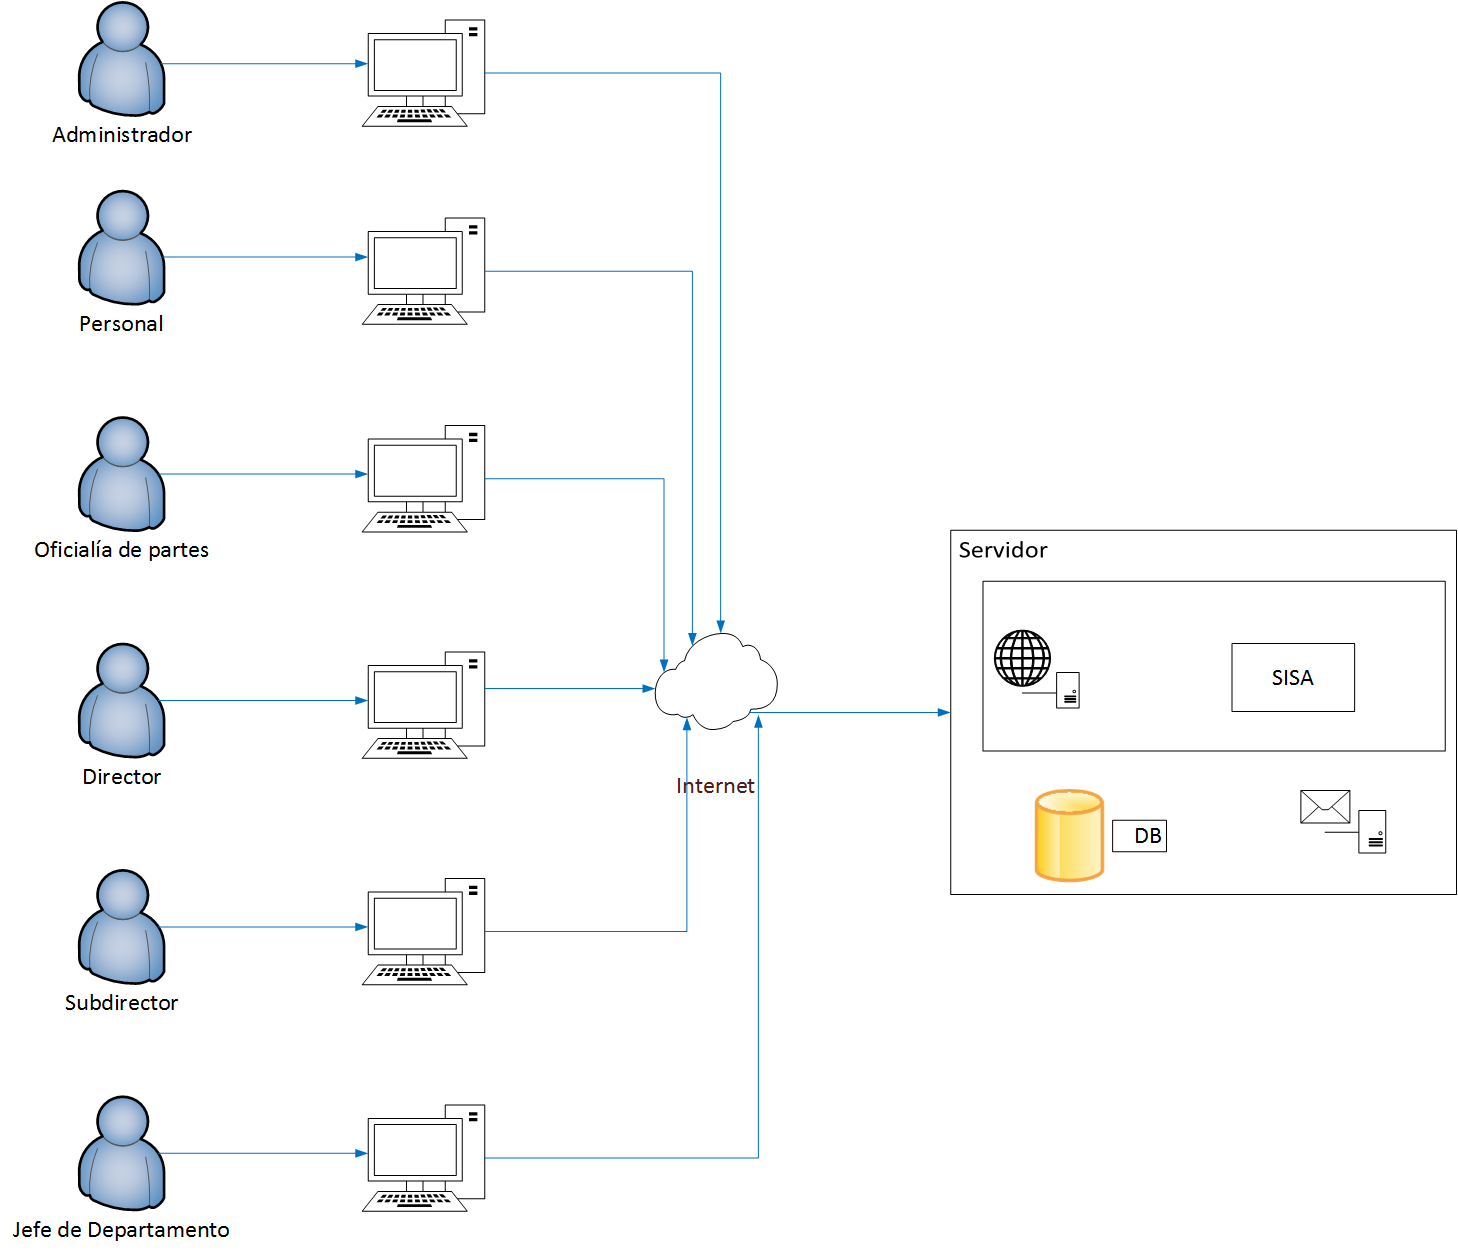
\includegraphics[width=0.8\textwidth]{images/propuesta/arquitectura}
		\caption{Arquitectura de la Aplicación.}
		\label{arquitectura}
	\end{figure}
	
\subsubsection{Hardware}

Dentro del hardware se requiere que el CMPL cuente con:
\begin{enumerate}
	\item Un servidor para que de el servicio a las computadoras, aloje la aplicación así como los registros de la correspondencia y se hagan los respaldos. Este servidor deberá contar con: 
	\begin{itemize}
		\item Al menos con 500 GB de disco duro.
		\item Un monitor.
		\item Un teclado.
		\item Un mouse.
		\item Al menos 8 GB en memoria RAM.
		\item Un procesador Intel Xeon.
	\end{itemize}
	\item Cada trabajador deberá contar con una computadora ya sea de escritorio o laptop con: 
	\begin{itemize}
		\item Al menos 256 GB de disco duro.
		\item 2 GB en memoria RAM.
		\item Un procesador Intel Quad Core. 
	\end{itemize}
\end{enumerate}

\subsubsection{Software}
El software que requiere es: 
\begin{enumerate}
	\item Un sistema operativo tanto para el servidor como las computadoras.
	\item Un navegador de internet.
	\item Un gestor de base de datos.
	\item Un servidor de correos.
	\item Un servidor web.
\end{enumerate}
\subsubsection{Servicios}

Por último se requiere de los siquientes servicios: 
\begin{itemize}
	\item Energía eléctrica o una planta de luz para que cuando se vaya la luz el servidor siga operando.
	\item Aire acondicionado: para que no se caliente el servidor.
	\item Site: para colocar el servidor.
	\item Seguridad física: para que ninguna persona diferente al jefe del departamento de sistemas y banco de datos modifique la configuración del servidor.
	\item Servicio web: para que los usuarios accedan a la aplicación. 
	\item Conexión a internet.
\end{itemize} 

%%%%%%%%%% PROCEDIMIENTO %%%%%%%%%%%%
%%%%%%%%%%%%%%%%%%%%%%%%%%%%%%%%%%%%%
\subsection{Procedimiento}
Con esta propuesta se mejora el procedimiento presentado en el capitulo 1, las principales mejoras son:

\begin{figure}[htbp!]
		\centering
			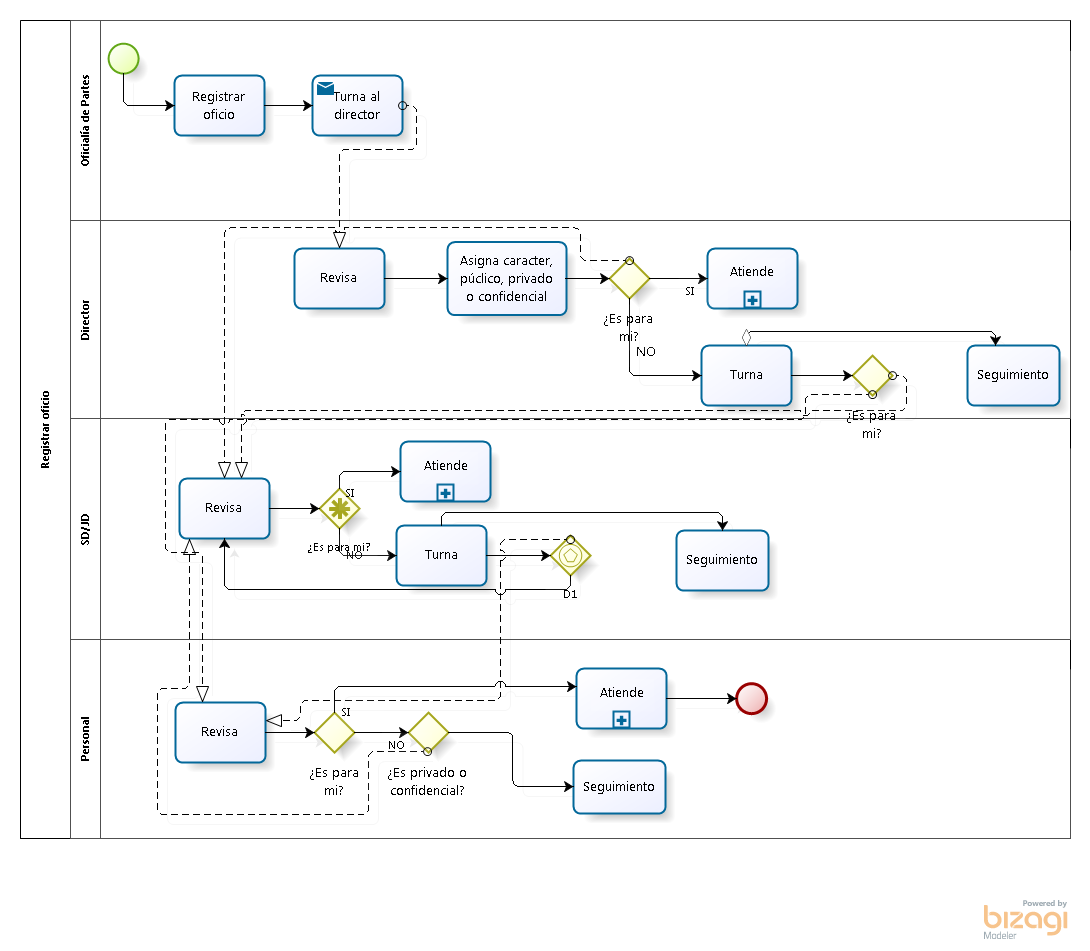
\includegraphics[width=0.8\textwidth]{images/propuesta/registrooficio}
		\caption{Procedimiento de recepción.}
		\label{Registro oficio}
	\end{figure}
	
\begin{itemize}
	\item Alertas al usuario: cuando el usuario este utilizando la aplicación está mostrará los asuntos que no ha atendido. 
	\item Notificaciones al correo: una vez que se turne un oficio, se enviará un correo electrónico al usuario diciendo que tiene un nuevo asunto por atender. 
	\item Respaldos: el administrador podrá realizar los respaldos de todos los registros de la corespondencia así como los documentos digitales.
	\item Seguimiento: el seguimiento de la correspondencia comprende varios estados...
\end{itemize}


%%%%%%%%%% INFORMACION %%%%%%%%%%%%%%
%%%%%%%%%%%%%%%%%%%%%%%%%%%%%%%%%%%%%
\subsection{Información}

Para la información a manejar dentro de la aplicación de manera general se comtempla manejar la información de:
\begin{itemize}
	\item Usuarios: Nombre completo, departamento al que pertenece, rol que desempeña dentro de la aplicación, contraseña y correo electrónico.
	\item Oficio entrante: número de oficio, fecha de redacción, área que emite, emisor, cargo del emisor, destinatario, cargo del destinatario, dependencia, asunto, fecha de acuse, nombre de quien entrega, si requiere o no respuesta, a quien se le turnó, a quien se le envió copia y si tiene documentos adjuntos. Además contará con un selector de archivos que permite la carga del documento escaneado en formato PDF y adjuntarlo al registro.
	\item Oficio saliente: número de oficio, fecha de redacción, área que emite, emisor, cargo del emisor, destinatario, cargo del destinatario, dependencia, asunto, fecha de acuse, nombre de quien entrega, si es respuesta a un oficio anterior y si tiene documentos adjuntos.
	\item Memorándum: fecha de redacción, destinatario, cargo del destinatario, departamento, asunto, área que emite, emisor, cargo del emisor, si require respuesta. 
\end{itemize}

%%%%%%%%%% PROPIEDADES DE SW %%%%%%%%
%%%%%%%%%%%%%%%%%%%%%%%%%%%%%%%%%%%%%
\subsection{Propiedades de software}

\textbf{Confiabilidad\\}
La confiabilidad de un sistema es la probabilidad de que el sistema realizará su funcionalidad bajo los limites de diseño especificados, sin fallo, durante un periodo de tiempo determinado. \\

\textbf{Disponibilidad\\}
La disponibilidad es la probabilidad de que el sistema esta operando en un tiempo particular.\\ 

\textbf{Robustes\\}
Un sistema de software es robusto si es capaz de responder adecuadamente a las condiciones de tiempo de ejecución no anticipados.\\


%%%% INTERACCION CON EL USUARIO %%%%%
%%%%%%%%%%%%%%%%%%%%%%%%%%%%%%%%%%%%%
\subsection{Interacción con el usuario}

La interacción de la aplicación con el usuario será mediante pantallas con formularios, mensajes de confirmación, alertas. 
%Cuenta con una pantalla que tiene un formulario de autenticación donde se le solicita al usuario su correo institucional y su contraseña. Cuando el usuario ingresa sus credenciales la aplicación verifica su correo y su contraseña; si existen entonces la aplicación muestra la pantalla principal de acuerdo al tipo de usuario que sea. En caso contrario, la aplicación regresa a la pantalla de autenticación con un mensaje de error diciendo que los datos introducidos no son válidos.

\section{Metodología}

La metodología que se utiliza para el desarrollo de este trabajo es Espiral, la cual consiste en hacer un conjunto de actividades en cada iteración las cuales no tienen prioridad sino que se eligen comenzando por la iteración anterior.\\

Para este proyecto se realizarán 4 iteraciones, en esta primera fase de evaluación se realizaron las primeras dos iteraciones. La primera iteración consistió en investigar y probar  diferentes tecnologías para desarrollar el proyecto tanto hardware como software y una vez hecho se configuraron las máquinas a utilizar y el servidor del CMPL. \\
La segunda iteración se realizó el análisis, diseño y desarrollo de la problemática, se realizaron las primeras pantallas.\\

parrafo de cierre 
%\item Que la aplicación controle el acceso de los usuarios restringiendo el uso de aplicación a la información y funciones que le corresponden.